% Template for ICASSP-2019 paper; to be used with:
%          spconf.sty  - ICASSP/ICIP LaTeX style file, and
%          IEEEbib.bst - IEEE bibliography style file.
% --------------------------------------------------------------------------
\documentclass{article}
\usepackage{spconf,amsmath,graphicx,epstopdf,float}

% Example definitions.
% --------------------
\def\x{{\mathbf x}}
\def\L{{\cal L}}

\title{Multi-scale Defect Detection Network for Tire X-ray Images}


%\name{Ren Wang{\rm\textsuperscript{1,2}}, Qiang Guo{\rm\textsuperscript{1,2}}, Shanmei Lu{\rm\textsuperscript{1,2}},  Caiming Zhang{\rm\textsuperscript{3}}}
\name{Ren Wang{\rm\textsuperscript{1,2}}, Qiang Guo{\rm\textsuperscript{1,2}},  Caiming Zhang{\rm\textsuperscript{3}}}
%\name{Ren Wang{\rm\textsuperscript{1,2}}}
\address{\textsuperscript{1}School of Computer Science and Technology, \\Shandong University of Finance and Economics, Jinan, China\\
        \textsuperscript{2}Shandong Provincial Key Laboratory of Digital Media Technology, Jinan, China\\
        \textsuperscript{3}Software College, Shandong University, Jinan, China}


\begin{document}
%\ninept

\maketitle

\begin{abstract}
Though automatic detection method has been tremendous improved, with the development of deep learning. Defect detection in many industrial processes is one of the remaining challenging tasks due to the diversity of products. In this work, we focus on detection tasks in tire industry and develop a {\it Multi-scale Defect Detection Network (MDDN)}, which contains two parallel sub-networks to capture multi-scale defect features. Specifically, high-abstracted semantic features containing defect shapes and locations are mined via a {\it Semantic-aware sub-network}, simplified by an off-the-shelf fully convolutional network. Furthermore, to complement the details filtered by the sub-sampling, a novel {\it Texture-aware Sub-network} is used to cover edge features and small defects as much as possible. Finally, pixel-wised detection results are obtained by fusing features with semantic and texture information. Extensive experiments demonstrate that {\it MDDN} can produce comparable results and achieve significantly performance improvement in small tire defects detection.
\end{abstract}

\begin{keywords}
Defect detection, Fully convolutional network, Semantic segmentation, Multi-scale context
\end{keywords}

\section{Introduction}
\label{sec:intro}
Automatic defect detection, used to improve quality and accelerate production, has become an indispensable part in industrial processes \cite{kumar2008computer,li2016deformable,ghorai2012automatic}. Especially in tire manufacturing, numerous detection algorithms have been proposed \cite{zhang2013texture,zhang2018tire,xiang2014dictionary} and aroused extensive attention recently. In most real-world applications, tire defect detection is first carried out by deriving the defective region from tire X-ray images, which contains various types of defects caused by unclean raw materials and undesired manufacturing facilities \cite{guo2016defect}. Then, defective products are hierarchical processed according to the location and area of defects. Due to unique properties of the tire X-ray image, for instance complexity and low-quality, illustrated in previous study \cite{zhang2013defect,wang2019tire}, most inspection processes are performed by human observers, which increases the risk and reduces the efficiency. Therefore, tire defect detection remains one of the most challenging inspection tasks.
\begin{figure}[t]
  \centering
  \centerline{\includegraphics[width=0.5\textwidth]{pic1.eps}}
  \caption{(a)shows the image pyramids. (b) indicates in-network feature hierarchies. Prediction results can be derived from each layer. (c) represents multi-size tire image patches, which can increase the relative scale of small defects and backgrounds. (d) illustrates that the semantic information is more easily retained in tire image peaches by comparison.}
\end{figure}
\begin{figure*}[t]
  \centering
  \centerline{\includegraphics[width=0.86\textwidth]{pic2-3.eps}}
  \caption{Overall architecture of the proposed MDDN. }
\end{figure*}

At present, existing computer vision based detection methods are mostly devoted to distinguishing difference between defective regions and background (defective-free regions). A key issue for such methods is feature extraction. Guo {\it et al}. \cite{guo2012tire} proposed a component decomposition based method to detect tire defects, which separated the background from the image by means of two designed filters. Then through an adaptive thresholding processing, defects were derived from the residual image. Besides, Independent component analysis was also used for defect detection tasks \cite{cui2016defect,cui2016novel}. A major disadvantage of these fundamental methods is the limitation of the information contained in low-level clues and domain features. To address the limitation, Zhang {\it et al}. \cite{zhang2013defect,zhang2015automatic} introduced mulit-scale wavelet and curvelet transform in detection tasks respectively. Furthermore, optimized edge detection and total variation algorithm are used to achieve more accurate results \cite{yan2013detection}. However, the representation capability of fixed kernels is not comprehensive enough. Moreover, transform processes are computationally expensive. Recently, Cui {\it et al}. \cite{cui2018tire} attempted to classify tire defects by means of deep convolutional networks (ConvNets), which has outstanding performance in the recognition and segmentation tasks of natural images. With the excellent feature extraction capability of the ConvNet, Wang {\it et al}. \cite{wang2019tire} further implemented the detection and segmentation in tire images by a fully convolutional network (FCN) \cite{long2015fully}. However, due to the existence of pooling layers, FCN is not sensitive to small defects and edge details, which is similar to that in dealing with natural image segmentation tasks.



To overcome these shortcomings, many methods have been proposed in benchmark datasets. Most of them are based on multi-scale strategies and can be roughly classifified into image pyramids and in-network feature hierarchies. Image pyramids were directly scaled to get multi-scale images and extensively used in the era of hand-crafted features \cite{lowe2004distinctive,dalal2005histograms}, as shown in Figure 1(a). Even if the crafted features have largely been replaced by self-learning features, multi-scale testings on the image pyramid are still used to verify the adaptability and robustness ({\it e.g.}, \cite{he2016deep}). Nevertheless, image pyramid based methods is impractical for real applications due to the considerable increase in inference time. In-network feature hierarchies are formed by the forward propagation within deep ConvNets. Through several of sub-sampling layers, in-network hierarchies produce feature maps of different spatial resolutions, with an multi-scale and pyramid shape\cite{lin2017feature}. By fusing these multi-scale feature maps, features in shallow and deep layers can be perceived. The Single Shot Detector (SSD) \cite{liu2016ssd} is one of the first attempts at combining predictions from these features maps to detect objects of various sizes. Generally, shallow features are used to predict small objects, and deep features with large receptive fields are used to detect large objects. However, the lack of semantic information is harmful to the detection of small targets in shallow layers. Another fusing way can effectively address this problem by concatenating multi-scale features and detecting on top of the expanded feature maps, as shown by the red line in Figure 1b[]. For example, FCN defined a skip architecture to produce more accurate segmentation. Similar top-down skip architectures are popular in recent research\cite{newell2016stacked,ghiasi2016laplacian}. There exists a basic problem that it is still not enough to mine the detail texture in these structures\cite{zhou2018scale}. Bai {\it et al}. proposed a novel multi-task generative adversarial network (MTGAN), which improve the detection performance by up-sampling a small object to a larger scale using super-resolution.

Inspired by MTGAN, we construct a end-to-end network named Multi-scale Defect Detection Network (MDDN) consisting of a semantic-aware sub-network and a texture-aware sub-network.
To detect small tire defects, image patches \cite{bai2018sod,chen2016attention} are fed in the texture-aware sub-network. Unlike natural image patches, defects (objects) are still significant and discernible in the tire image patches, illustrated in Figure 1(d). In addition, as shown in Figure 1(c), the proportion of defects in a 256 $\times$ 256 tire image increases from 124/65535 to 124/4096, which is advantageous for better capturing of detailed information.



%\Figure[t!][width=0.86\textwidth]{test1.eps}
%{Detection results of several benchmark architecture. (a) shows input tire images with different defects. From top to bottom, the first four are tire sidewall images, which involve following defect types: impurity, overlap, slack, bubble. The last two are tire tread images, which involve overlaps. (b) indicates ground truths obtained by manual marking. (c),(d),(e) and (f) are detection results using AlexNet, VGG11, VGG13 and VGG16 as the basic architecture, respectively. \label{fig1}}

\section{Multi-scale Defect Detection Network}
\label{sec:format}

Our deep network aims to improve the accuracy of tire defect detection, especially for edge detail and small defects. To achieve this goal, on the one hand, the proposed MDDN combines deep layer features with low-level clues through two parallel sub-networks. Among them, the semantic-aware network is adopted to mine abstract semantic features including shape and location information, which is simplified by FCN \cite{long2015fully}, a deep network that has outstanding performance in solving the semantic segmentation problems with natural images. Furthermore, in order to supplement the detailed information filtered during the extraction of high-level semantics, a novel texture-aware network is developed to attempt to cover more shallow detail information without increasing computational complexity. On the other hand, owing to the characteristics of the tire images, a variety of data preprocessing methods are used to enhance performance for the two sub-networks. In the following subsections, we describe these networks and strategies in detail.

\subsection{Semantic-aware sub-network}
\label{Semantic-aware sub-network}
The proposed approach captures the desired high-level semantics of defects using an architectural design similar to the well-known FCN-VGG16 (a FCN with VGG16 as the basic framework), which has been proven to be viable in tire defect detection tasks. At first, a stack of convolution layers and max pooling layers are used repeatedly to obtain the most representative information in tire images. Each fully connected layer in the VGG16 is then replaced by a special convolutional layer to retain sufficient spatial information. Finally, prediction results with the same size as input images are derived by up-sampling these spatial feature maps. We simplify an off-the-shelf FCN-VGG16 into a binary-classification and pixel-wise detection model. Moreover, we normalize the parameters of convolutional layers, such as both padding and stride are set to 1 and the convolution kernel size is set to 3 $\times$ 3, and remove the crop layers to reduce noise and increase the detection efficiency.

Although the learned filter in VGG network are excellent generic visual descriptors, it is originally trained for the purpose of object classification tasks. The existence of the five max pooling layers allows it to filter out the essential details while having the capability to mine global semantic information. Therefore, the FCN is not sensitive to the edge details detection, especially for small-sized defects.

\subsection{Texture-aware sub-network}
\label{Texture-aware sub-network}
As mentioned above, to complement the details filtered by pooling layers, a novel texture-aware network, in parallel with the semantic-aware network, is developed to obtain detailed clues in shallow layers. The texture-aware network employs 4 convolutional layers inspired by FSRCNN\cite{dong2016accelerating}, a network that is expert in handling precise visual tasks such as super-resolution. The first layer of convolution uses a 5 $\times$ 5 convolution kernel to extract the features of the input image. These features are directly used by later layers to increase computational complexity. Although these feature maps carrying a large amount of valuable information can be directly mapped by next layers, this leads to an increase in computational complexity. Therefore, the second convolutional layer uses a 1 $\times$ 1 convolution kernel to reduce computational cost and redundancy information, called shrinking. The latter two 3 $\times$ 3 convolutions are adopted to improve representation capability. Without the existence of pooling layers, detailed features can be completely retained. Meanwhile, the down-sampling capability of the shrinking layer in the channel dimension can both reduce redundant information and retain the spatial resolution.

In order to make the texture-aware network more robust to scale variations, images are preprocessed through multi-scale blocking and scaling strategies. Generally, in natural image segmentation tasks, the blocking operation first obtains object proposals[], and then finely segmentation in these regions. In contrast, tire images can be cropped evenly while retaining defect semantic information, due to the similarity of background textures. As shown in Figure 1c, the cropping and scaling essentially change the proportion of defects in training images. In this paper, we crop 4 and 16 blocks without overlap from each image, and consider scales of 0.5 and 1.5.


\subsection{Combination and training}
\label{Combination and training}

Although features extracted by the texture-aware network contain the essential details, the detection results derived from these features usually have a large amount of noise and a high false positive rate without the guidance of global semantics. Therefore, the fusion of semantic-aware networks and texture-aware networks is necessary. Semantic and texture feature maps are combined and fused in the channel dimension via a {\it concat} layer and a 1 $\times$ 1 convolution layer.

Since the two sub-networks use different input data and preprocessing methods, we first train the texture-aware network using the block data, and then train the entire network with fixed training texture-aware network parameters. As described in the previous subsections, owing to the characteristics of tire image textures, original images can be directly input during the test phase. And the end-to-end test results can be obtained. The experiment proves the effectiveness of this means.

\section{EXPERIMENTS}
\label{sec:pagestyle}
\subsection{Implementation details}
\label{Implementation details}
{\bf Dataset.} Our experimental dataset consists of 914 tire images including both sidewall and tread images. These images involve various defects such as metal impurities, bubbles, and overlaps. For semantic-aware networks, we consider flipping and mirroring to enhance the data. For texture-aware networks, cropping and scaling are used, as mentioned above.\\
{\bf Parameter Setting.} The proposed MDDN was coded with Python 3.5 in the Caffe framework. A GTX-1080 GPU and Intel Xeon-E5 3.40GHz CPU are used for both training and testing. The momentum parameter and weight decay were set to 0.99 and 0.0005 during training, respectively. Moreover, semantic-aware network is implemented on the public FCN code, and the parameters of the texture-aware network are randomly initialized. \\
{\bf Metrics.} We adopt the widely used metrics in instance segmentation community, including intersection over union(IOU) and pixel accuracy (PA). The former can represent the accuracy of location. And the latter indicates the ratio of the correct labeled pixels to the total pixels, which reflects the pixel-level accuracy of the detection results.


\begin{figure*}[t]
  \centering
  \centerline{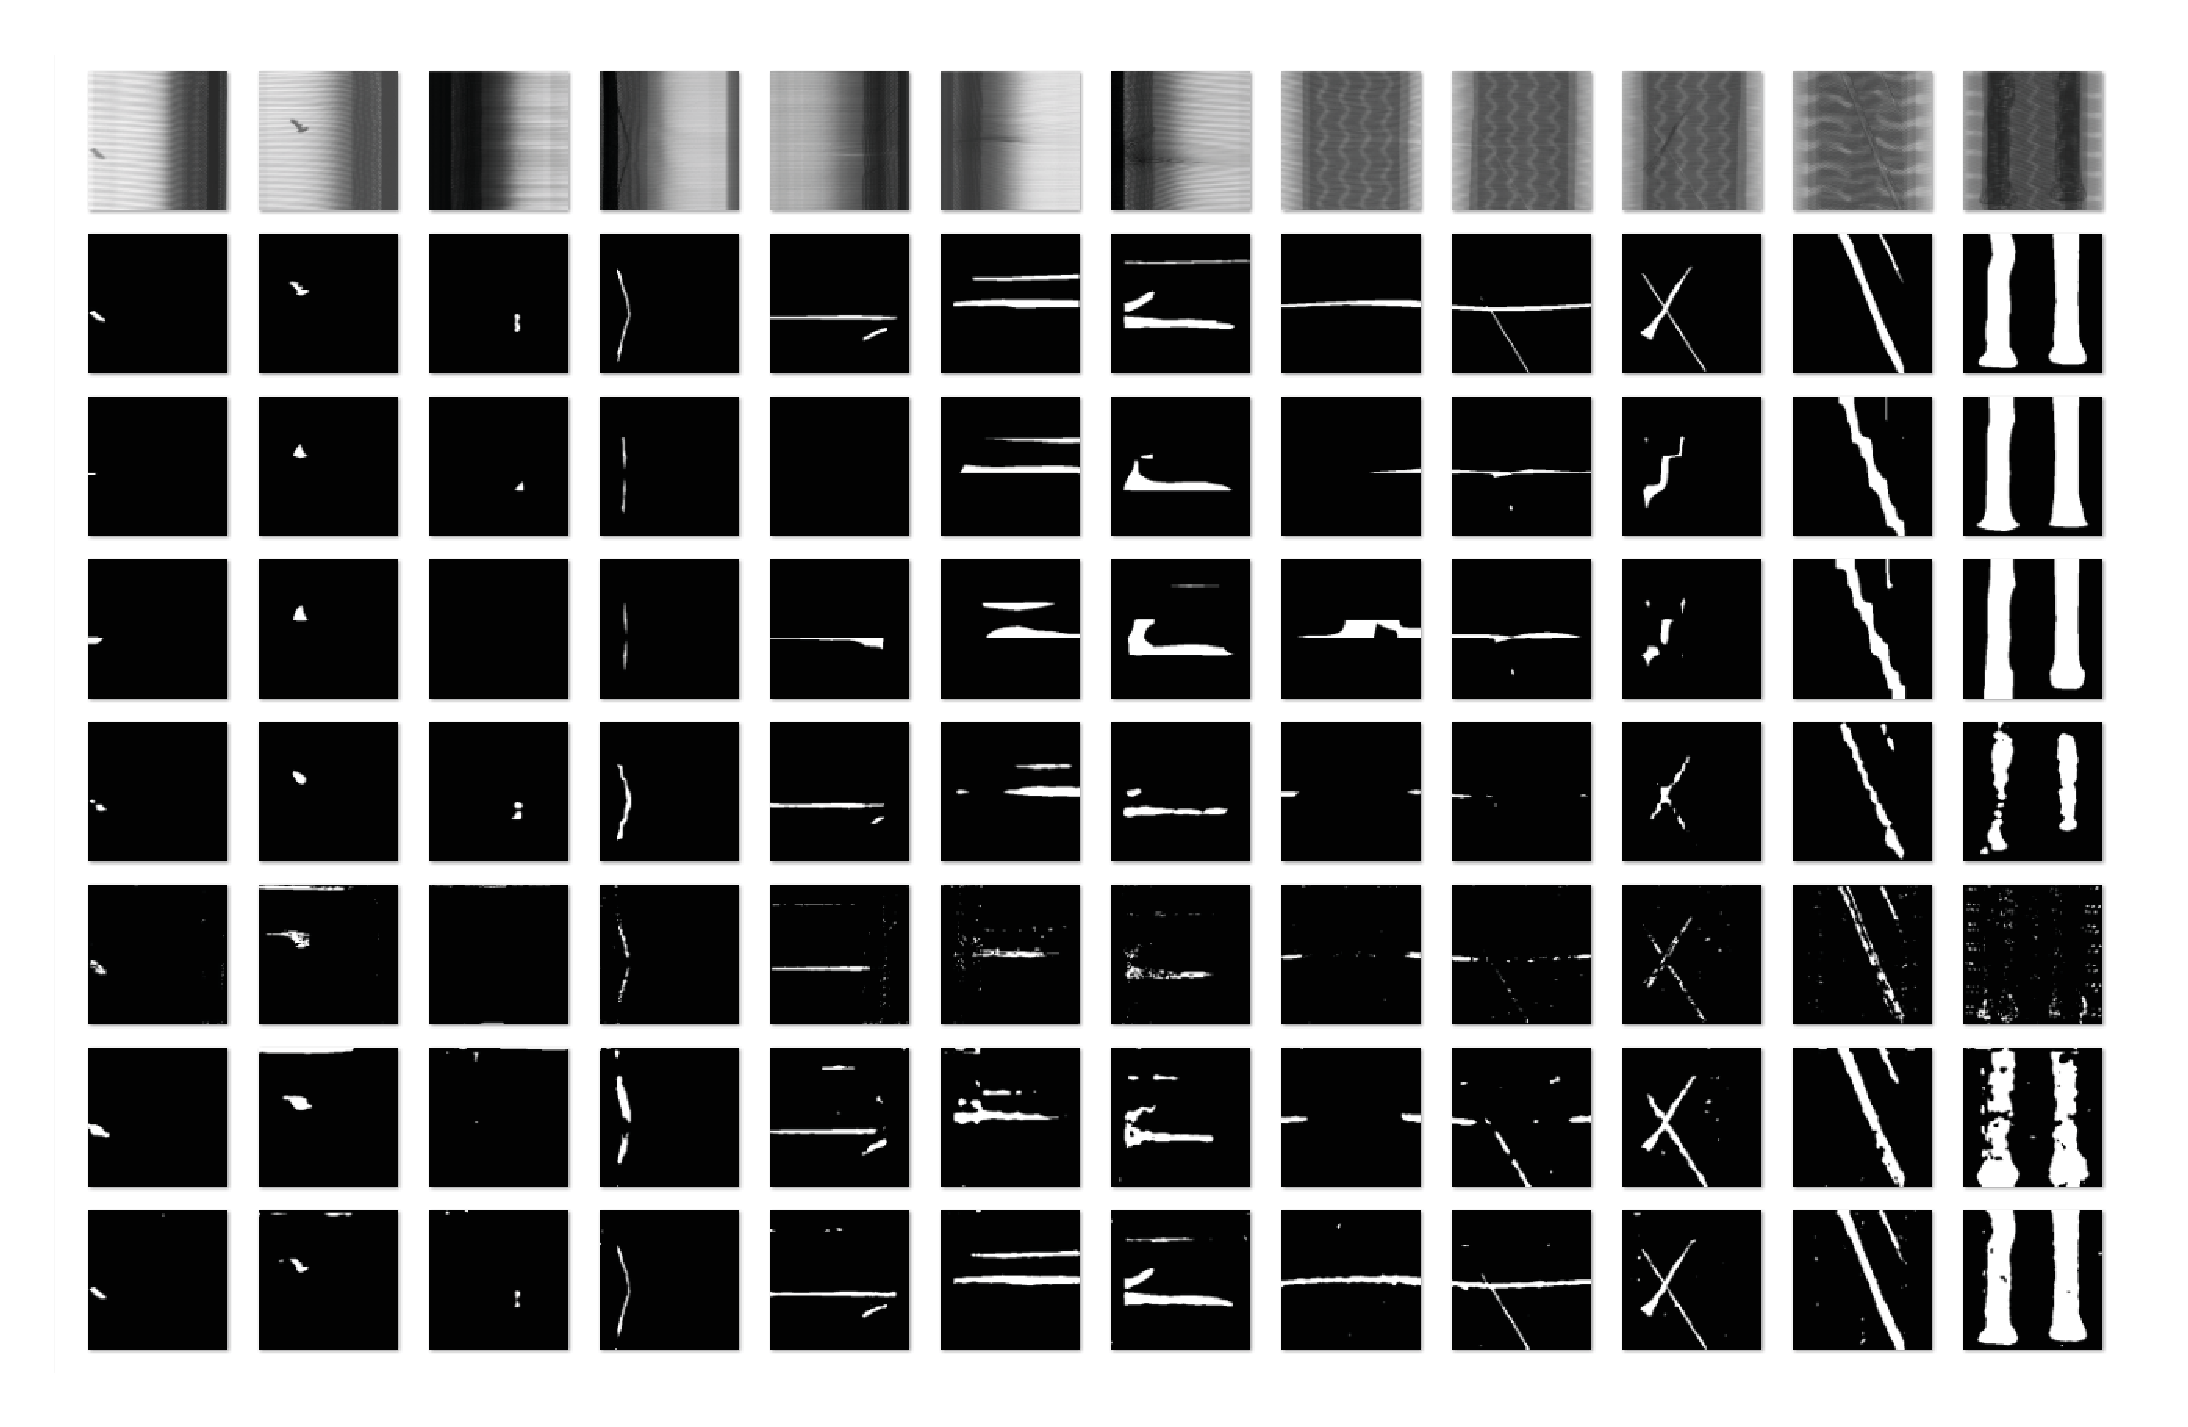
\includegraphics[width=0.95\textwidth]{pic3.eps}}
  \caption{Comparison of experimental results.}
\end{figure*}

\subsection{Ablation experiment}
\label{Ablation experiment}
In order to evaluate the parameter effectiveness of our proposed MDDN method, we conduct two groups of ablation experiments on the same data set. In one group, features learned by the semantic-aware network and the texture-aware network are used alone to detect defects. As the results shown in the figure **. The semantic-aware network can roughly detect the location and shape of the defect. The texture-aware network has a high false positive rate due to the large amount of noise in the extracted features. In another group, for the same network trained with blocks, we use the blocks and the original images for testing. The experimental results verify that tire blocks still has relatively complete semantic information.

\subsection{Comparison with state-of-the-art methods}
\label{state-of-the-art methods}
Comparison with state-of-the-art methods.Comparison with state-of-the-art methods.Comparison with state-of-the-art methods.Comparison with state-of-the-art methods.
Comparison with state-of-the-art methods.Comparison with state-of-the-art methods.Comparison with state-of-the-art methods.Comparison with state-of-the-art methods.
Comparison with state-of-the-art methods.Comparison with state-of-the-art methods.Comparison with state-of-the-art methods.Comparison with state-of-the-art methods.
Comparison with state-of-the-art methods.Comparison with state-of-the-art methods.Comparison with state-of-the-art methods.Comparison with state-of-the-art methods.
Comparison with state-of-the-art methods.Comparison with state-of-the-art methods.Comparison with state-of-the-art methods.

%%%%\begin{figure}[htb]

%%%%\begin{minipage}[b]{1.0\linewidth}
%%%%  \centering
%%%%  \centerline{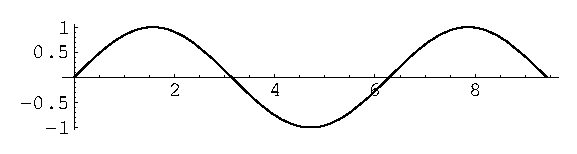
\includegraphics[width=8.5cm]{image1.eps}}
%  \vspace{2.0cm}
%%%%  \centerline{(a) Result 1}\medskip
%%%%\end{minipage}
%
%%%%\begin{minipage}[b]{.48\linewidth}
%%%%  \centering
%%%%  \centerline{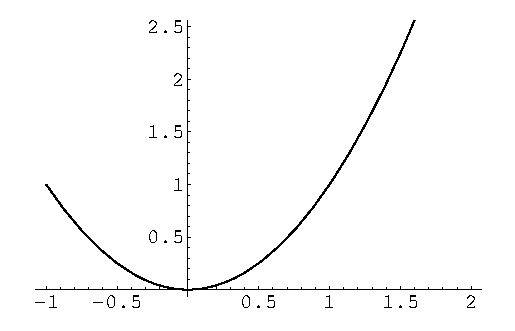
\includegraphics[width=4.0cm]{image3.eps}}
%  \vspace{1.5cm}
%%%%  \centerline{(b) Results 3}\medskip
%%%%\end{minipage}
%%%%\hfill
%%%%\begin{minipage}[b]{0.48\linewidth}
%%%%  \centering
%%%%  \centerline{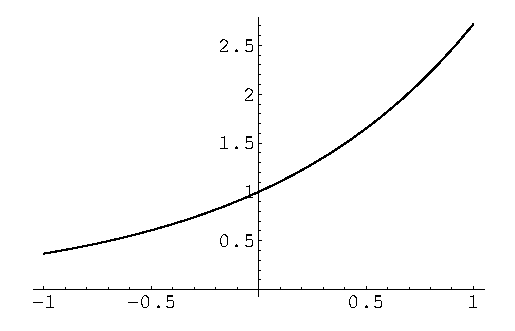
\includegraphics[width=4.0cm]{image4.eps}}
%  \vspace{1.5cm}
%%%%  \centerline{(c) Result 4}\medskip
%%%%\end{minipage}
%
%%%%\caption{Example of placing a figure with experimental results.}
%%%%\label{fig:res}
%
%%%%\end{figure}


% Below is an example of how to insert images. Delete the ``\vspace'' line,
% uncomment the preceding line ``\centerline...'' and replace ``imageX.ps''
% with a suitable PostScript file name.
% -------------------------------------------------------------------------


\section{CONCLUSION}
\label{sec:typestyle}

In this paper, we proposed a MDDN model for detailed tire defect detection tasks. Through combining a semantic-aware network and a novel texture-aware network, MDDN can preserve the necessary detail features while mining the semantic information hidden in deep layers. We showed that an increase in the proportion of defective areas is critical for small defect detection. In addition, we have experimentally verified that the blocking strategy can effectively enhance the dataset and retain detailed information, in tire images. The experiments demonstrate that our MDDN has significantly improved over the existing tire defect detecting methods, and can produce more accurate small defect detection results. The future work includes reducing noises in the texture-aware network and increasing detection speed.

% To start a new column (but not a new page) and help balance the last-page
% column length use \vfill\pagebreak.
% -------------------------------------------------------------------------
%\vfill
%\pagebreak

\vfill\pagebreak




% References should be produced using the bibtex program from suitable
% BiBTeX files (here: strings, refs, manuals). The IEEEbib.bst bibliography
% style file from IEEE produces unsorted bibliography list.
% -------------------------------------------------------------------------
\bibliographystyle{IEEEbib}
\bibliography{strings,refs}

\end{document}
